\subsection{Natureza da função beta}
Qual é a forma desejada de $\beta(s)$? Já foi visto que, pelo menos em alguns aspectos, pequenos valores de $\beta$ (focalização forte) são desejados -- tal que $\beta$ seja razoavelmente uniforme. Infelizmente, pequenos valores de $\beta$ só podem ser obtidos alternando o gradiente de focalização, o que tende a gerar oscilações razoavelmente grandes em $\beta$. Além disso, pequenos valores de $\beta$ implicam em grandes valores de $\nu$, o que pode gerar maiores dificuldades ao se lidar com as ressonâncias. Normalmente, $\beta$ tem um valor típico entre $1/2$ e $1/6$ do raio de curvatura $R$, não tendo, assim, oscilações muito extremas.

A função betatron é definida pela função singular, contínua a qual sua raiz quadrada satisfaz
\begin{align}
	\zeta'' = -K(s)\zeta + \frac{1}{\zeta^3}\label{eq:2.74}
\end{align}
onde $K(s)$ é a função de focalização. Tipicamente, os anéis modernos são feitos de vários segmentos nos quais a função $K(s)$ é constante, podendo ser nula, positiva ou negativa.

A imposição de que $\zeta(s)$ tem que ser periódica, juntamente com o termo não linear $1/\zeta^3$, gera uma especificação única -- incluindo a escala. A função $\zeta(s)$ é a função própria da equação \eqref{eq:2.74} e, por causa da não-linearidade, não existe uma normalização arbitrária da amplitude.

Fazendo uma análise dimensional, espera-se que $\zeta$ tenha uma dimensão $|K|^\frac{-1}{4}$, ou que $\beta$ tenha uma dimensão $|K|^\frac{-1}{2}$. (Relembrando que $1/\beta$ é como se fosse a frequência da oscilação, é esperado que esta esteja de acordo com a raiz da constante da força restauradora). Para uma dada geometria do campo, esta lei de escala é grosseiramente verdadeira. Ela é estritamente verdadeira se a escala do comprimento da geometria de focalização é escalada em $|K|^\frac{-1}{2}$, o que geralmente é válido em campos guia bem projetados.

Em uma região de $s$ em que $K(s)$ é constante, , a equação \eqref{eq:2.74} tem a forma da equação de movimento de uma partícula sob o efeito de uma força restauradora $-K\zeta$ e uma força repulsiva $1/\zeta^3$. Ou, da mesma forma, uma partícula que se move com uma energia potencial proporcional a
\begin{align}
	K\zeta^2 + \frac{1}{\zeta^2}
\end{align}
(O segundo termo é como se fosse uma barreira centrífuga!). O formato do potencial efetivo é mostrado na \autoref{fig:fig16} para os três casos de $K$.

\begin{figure}[!htb]
	\centering
	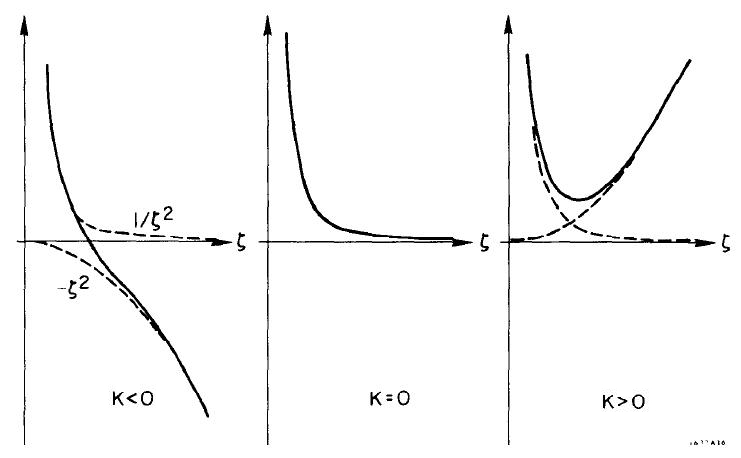
\includegraphics[width=0.9\linewidth]{./Figuras/fig16.jpeg}
	\caption{Funções potenciais efetivas para $\zeta$. Retirado de \cite{sands1970physics}.}
	\label{fig:fig16}
\end{figure}

Em qualquer região onde $K\leq 0$, a aceleração em $\zeta$ (o desvio da partícula de referência) é sempre positiva; e $\zeta$ direcionado sempre para valores maiores -- ou, claro, dar a volta caso sua velocidade inicial seja na direção da origem de $\zeta$. Para $K$ negativo, a força direcional é, em grandes valores de $\zeta$, proporcional ao tamanho de $K$. Por outro lado, em qualquer região onde $K>0$, haverá um potencial estável e, quando $\zeta$ assume grandes valores, sempre há uma força direcionando $\zeta$ para a origem.

Também é qualitativamente aparente que possa existir soluções estáveis onde $\zeta(s)$ entra numa região onde $K<0$ movendo-se em direção à origem e muda de sentido devido à força de repulsão apenas para ser mandado na direção da origem novamente pela força de atração numa região posterior onde $K>0$. Para um K periódico como o da \autoref{fig:fig17}(a), deve-se esperar uma solução para $\zeta(s)$ como a curva representada na parte (b). A solução exibe uma importante característica geral da função $\zeta$: seu máximo ocorre em seções focalizadoras -- onde $K>0$ -- e seu mínimo ocorre em seções desfocalizadoras ou neutras -- onde $K \leq 0$.

\begin{figure}[!htb]
	\centering
	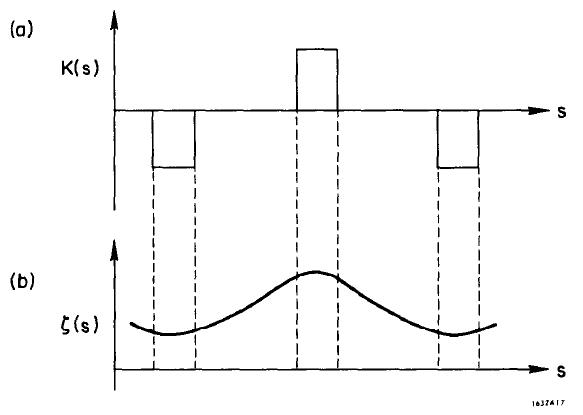
\includegraphics[width=0.7\linewidth]{./Figuras/fig17.jpeg}
	\caption{Forma da função $\zeta(s)$ com uma função de focalização $K(s)$ periódica. Retirado de \cite{sands1970physics}.}
	\label{fig:fig17}
\end{figure}

Também é evidente que para um determinado espaçamento com diferentes valores de $K$, se a magnitude de $K$ aumenta, a amplitude das oscilações irá crescer rapidamente. Menos evidente é o fato de que, conforme a escala de $K$ aumenta, chegará num ponto em que uma solução estável -- isto é, periódica -- para $\zeta(s)$ não existirá mais. Então a força de focalização (magnitude de $K$) e o espaçamento entre os elementos deve ser ajustado em conjunto, gerando a estrutura óptica do anel -- mais conhecido como \textit{lattice}, uma palavra para indicar a geometria dos segmentos.

Pode ocorrer o questionamento "Por que não apenas tem valores negativos de $K$ em todo $s$? Claramente a estabilidade de $\zeta$ é garantida". Isto não é possível pois quando $K$ é negativo em $x$, ele é automaticamente positivo em $z$, e vice-versa. Detsa forma, fica claro que é necessário alternar o gradiente de focalização.

Também deve estar evidente que as oscilações de $\zeta(s)$ -- e, portanto, de $\beta(s)$ -- estarão fora de fase na duas coordenadas transversais: $x$ e $z$. Quando $\zeta)x$ estiver em seu máximo, $\zeta_z$ estará em seu mínimo. Este comportamento é válido até nas estruturas mais complexas -- apesar de não ser totalmente verdade que $\zeta_x$ e $\zeta_z$ tem totalmente a mesma forma. 
%Na \autoref{fig:fig18} está um exemplo das funções $\zeta_x$ e $\zeta_z$.

%\begin{figure}[!htb]
%	\centering
%	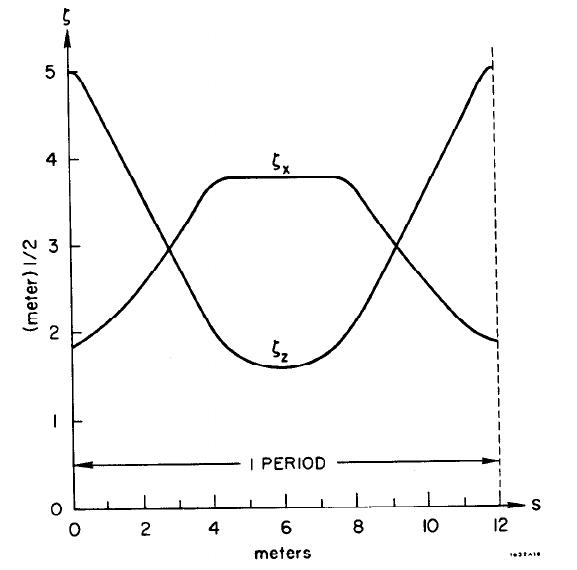
\includegraphics[width=0.7\linewidth]{./Figuras/fig18.jpeg}
%	\caption{Funções $\zeta_x$ e $\zeta_z$ de um campo guia. Retirado de \cite{sands1970physics}.}
%	\label{fig:fig18}
%\end{figure}

É intuitivo relacionar a função betatron $\beta(s)$ com a \textit{sine-like trajectory} definida na \autoref{sec:2.6}. A \textit{sine-like trajectory} $S(s,s_0)$ associada com a coordenada $s_0$ é a trajetória que começa em $s_0$ com deslocamento nulo e inclinação unitária. Esta pode ser expressa em termos da oscilação pseudo-harmônica dada pela equação \eqref{eq:2.43} substituindo $a=\sqrt{\beta(s_0)}$ e $\vartheta=\pi/2 + \varphi(s_0)$:
\begin{align}
	S(s,s_0) = \sqrt{\beta(s_0)\beta(s)}\ sen \left(\int\limits_{s_0}^{s} \frac{d\bar{s}}{\beta(\bar{s})}\right)
\end{align}
\begin{proof}
	Seja a trajetória dada pela equação \eqref{eq:2.43}:
	\begin{align*}
		x(s) = a\sqrt{\beta(s)}\ cos(\varphi(s)-\vartheta)
	\end{align*}
	com
	\begin{align*}
		\varphi(s) = \int\limits_{0}^{s} \frac{d\bar{s}}{\beta(\bar{s})}
	\end{align*}
	Substituindo $\vartheta=\pi/2 - \varphi(s_0)$:
	\begin{align*}
		x(s) &= a\sqrt{\beta(s)}\ cos(\varphi(s)-(\pi/2 + \varphi(s_0)))\\
			 &= a\sqrt{\beta(s)}\ sen(\varphi(s) - \varphi(s_0))
	\end{align*}
	Pela definição de $\varphi$,
	\begin{align*}
		x(s) &= a\sqrt{\beta(s)}\ sen\left(\int\limits_{0}^{s} \frac{d\bar{s}}{\beta(\bar{s})} - \int\limits_{0}^{s_0} \frac{d\bar{s}}{\beta(\bar{s})}\right)\\
			 &= a\sqrt{\beta(s)}\ sen\left(\int\limits_{s_0}^{s} \frac{d\bar{s}}{\beta(\bar{s})}\right)
	\end{align*}
	Substituindo $a=\sqrt{\beta(s_0)}$:
	\begin{align*}
		x(s) &= \sqrt{\beta(s_0)}\sqrt{\beta(s)}\ sen\left(\int\limits_{s_0}^{s} \frac{d\bar{s}}{\beta(\bar{s})}\right)\\
			 &= \sqrt{\beta(s_0)\beta(s)}\ sen\left(\int\limits_{s_0}^{s} \frac{d\bar{s}}{\beta(\bar{s})}\right)\\
		\therefore S(s,s_0) &= \sqrt{\beta(s_0)\beta(s)}\ sen\left(\int\limits_{s_0}^{s} \frac{d\bar{s}}{\beta(\bar{s})}\right)
	\end{align*}
	Checando,
	\begin{align*}
		S(s_0,s_0) &= \sqrt{\beta(s_0)\beta(s_0)}\ sen\left(\int\limits_{s_0}^{s_0} \frac{d\bar{s}}{\beta(\bar{s})}\right)\\
				   &= \beta(s_0)\ sen(0)\\
				   &= 0\\
		S(s,s_0)' &= \left(\sqrt{\beta(s_0)\beta(s)}\ sen\left(\int\limits_{s_0}^{s} \frac{d\bar{s}}{\beta(\bar{s})}\right)\right)'\\
				  &= \left(\sqrt{\beta(s_0)\beta(s)}\right)'\ sen\left(\int\limits_{s_0}^{s} \frac{d\bar{s}}{\beta(\bar{s})}\right) + \sqrt{\beta(s_0)\beta(s)}\ \left(sen\left(\int\limits_{s_0}^{s} \frac{d\bar{s}}{\beta(\bar{s})}\right)\right)'\\
				  &= \frac{1}{2}\frac{1}{\sqrt{\beta(s_0)\beta(s)}}(\beta(s_0)\beta(s))'\ sen\left(\int\limits_{s_0}^{s} \frac{d\bar{s}}{\beta(\bar{s})}\right) + \sqrt{\beta(s_0)\beta(s)}\ cos\left(\int\limits_{s_0}^{s} \frac{d\bar{s}}{\beta(\bar{s})}\right) \frac{1}{\beta(s)}\\
		S(s_0,s_0)' &= \frac{1}{2}\frac{1}{\sqrt{\beta(s_0)\beta(s_0)}}(\beta(s_0)\beta(s_0))'\ sen\left(\int\limits_{s_0}^{s_0} \frac{d\bar{s}}{\beta(\bar{s})}\right) + \sqrt{\beta(s_0)\beta(s_0)}\ cos\left(\int\limits_{s_0}^{s_0} \frac{d\bar{s}}{\beta(\bar{s})}\right) \frac{1}{\beta(s_0)}\\
					&= \frac{1}{2}\frac{1}{\beta(s_0)}(\beta(s_0)\beta(s_0))'\ sen(0) + \beta(s_0)\ cos(0) \frac{1}{\beta(s_0)}\\
					&= 0 + \beta(s_0)\frac{1}{\beta(s_0)}\\
					&= 1
	\end{align*}
	c.q.d.
\end{proof}

Agora, considere o que acontecerá se esta trajetória senoidal for seguida por uma volta completa -- ou seja, $s=s_0+L$. A integral fica, pela equação \eqref{eq:2.60}, apenas $2\pi\nu$. Devido à periodicidade da função betatron, $\beta(s_0+L) = \beta(s_0)$. Então,
\begin{align}
	S(s_0+L,s_0) = \beta(s_0)\ sen(2\pi\nu)
\end{align}
e, como $\nu$ independe de $s_0$, pode-se escrever também
\begin{align}
	\beta(s) = \frac{S(s+L,s)}{sen(2\pi\nu)}\label{eq:2.77}
\end{align}
Assim, a função betatron em $s$ é, a menos de uma constante, apenas o desvio após uma revolução da \textit{sine-like trajectory} começando em $s$. Veja a \autoref{fig:fig19}.

\begin{figure}[!htb]
	\centering
	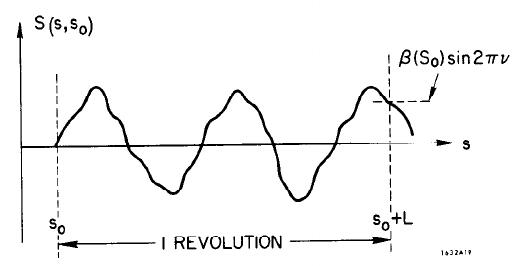
\includegraphics[width=0.8\linewidth]{./Figuras/fig19.jpeg}
	\caption{Relação entre $S(s,s_0)$ e $\beta(s_0)$. Retirado de \cite{sands1970physics}.}
	\label{fig:fig19}
\end{figure}

Pode-se obter uma outra prescrição para encontrar $\beta(s)$. Uma que precisa apenas do cálculo direto da \textit{sine-like trajectory} após uma revolução, começando em cada $s$.

O desvio obtido é proporcional a $\beta(s)$. Apenas resta determinar o fator de normalização $1/2\pi\nu$. Usando a definição de $\nu$ dada pela equação \eqref{eq:2.60}, juntamente com a equação \eqref{eq:2.77}, pode-se observar que a sintonia $\nu$ pode ser obtida como a solução da equação transcendental
\begin{align}
	\frac{2\pi\nu}{sen(2\pi\nu)} = \int\limits_{0}^{L} \frac{ds}{S(s+L,s)}
\end{align}
Então, conhecendo $S(s+L,s)$ para todo $s$, pode-se determinar $\beta(s)$ de forma única.

O cálculo de $S(s+L,s)$ pode ser efetuado por uma integração numérica da equação de movimento. Ou, para um campo guia uniforme, é também pode ser obtido utilizando o método matricial descrito na \autoref{sec:2.5}. Relembrando a equação \eqref{eq:2.37}, a \textit{sine-like trajectory} de $s_0$ para $s_0+L$ é apenas o elemento da primeira linha e da primeira coluna da matriz de transferência $\boldsymbol{M}(s,s_0)$ para a máquina completa, começando em cada $s_0$.

Também pode-se mostrar que a sintonia $\nu$ pode ser obtida pelo traço da matriz para o anel todo:
\begin{align}
	cos(2\pi\nu) = \frac{1}{2} Tr \boldsymbol{M}(s+L,s) = \frac{1}{2}[C(s+L,s) + S'(s+l,s)]
\end{align}
onde $C$ é a \textit{cosine-like trajectory}. Então, se $C$ e $S'$ são calculados assim como $S$, $\nu$ pode ser determinada e a equação \eqref{eq:2.77} pode ser obtida diretamente.

Pode-se escrever a equação diferencial \eqref{eq:2.74} de $\zeta$ em termos de $\beta$:
\begin{align}
	\frac{1}{2}\beta\beta'' - \frac{1}{4}\beta'^2 + K(s)\beta^2 = 1\label{eq:2.80}
\end{align}

\begin{proof}
	Seja a equação diferencial $\zeta'' = -K(s)\zeta + \frac{1}{\zeta^3}$. Substituindo $\zeta = \sqrt{\beta}$,
	\begin{align*}
		\sqrt{\beta}'' &= -K\sqrt{\beta} + \frac{1}{\sqrt{\beta}^3}\\
		\left(\beta^\frac{1}{2}\right)'' &= -K\beta^\frac{1}{2} + \frac{1}{\beta^\frac{3}{2}}\\
		\left(\beta^\frac{1}{2}\right)''\beta^\frac{3}{2} &+ K\beta^\frac{1}{2} \beta^\frac{3}{2} = 1\\
		\left(\beta^\frac{1}{2}\right)''\beta^\frac{3}{2} &+ K\beta^2 = 1
	\end{align*}
	Derivando,
	\begin{align*}
		\left(\beta^\frac{1}{2}\right)''\beta^\frac{3}{2} + K\beta^2 &= 1\\
		\left(\frac{1}{2}\beta^\frac{-1}{2}\beta'\right)'\beta^\frac{3}{2} + K\beta^2 &= 1\\
		\left(\left(\beta^\frac{-1}{2}\right)'\beta' + \left(\beta^\frac{-1}{2}\right)\beta''\right)\frac{1}{2}\beta^\frac{3}{2} + K\beta^2 &= 1\\
		\left(\frac{-1}{2}\beta^\frac{-3}{2}\beta'\beta' + \beta^\frac{-1}{2}\beta''\right)\frac{1}{2}\beta^\frac{3}{2} + K\beta^2 &= 1\\
		\frac{-1}{4}\beta'^2 + \frac{1}{2}\beta\beta'' + K\beta^2 &= 1
	\end{align*}
	c.q.d.
\end{proof}

A partir da equação \eqref{eq:2.80}, podem-se fazer algumas observações. Primeiramente, em um trecho reto do anel (sem campo magnético), $K(s)=0$ e a solução da equação \eqref{eq:2.80} é
\begin{align}
	\beta = \beta_0\left[1+\frac{(s-s_0)^2}{\beta_0^2}\right]
\end{align}
onde $s_0$ e $\beta_0$ são constantes adequadas. Se $\beta$ tem um ponto de mínimo em um trecho reto, então $\beta_0$ e $s_0$ são os valores de $\beta$ e $s$ neste mínimo. Sua forma é ilustrada na \autoref{fig:fig20}. Note que o coeficiente do termo quadrático é o inverso do valor de $\beta$ no seu ponto mínimo -- quanto menor for $\beta_0$. mais rápido é o aumento de $\beta$ com o aumento da distância do ponto de mínimo.

Finalmente, observe que em um segmente que $K$ é grande e $\beta'$ pequeno, a equação \eqref{eq:2.80} pode ser aproximada por
\begin{align}
	\beta'' = -2K\beta
\end{align}
Assim, $\beta$ é uma senoide ou uma exponencial dependendo do sinal de $K$.

\begin{figure}[!htb]
	\centering
	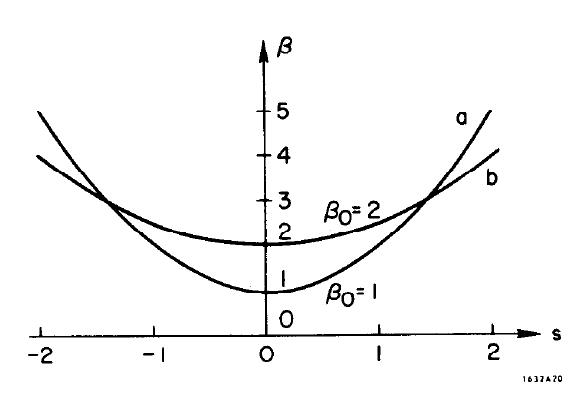
\includegraphics[width=0.8\linewidth]{./Figuras/fig20.jpeg}
	\caption{Variação de $\beta$ próximo do mínimo o qual ocorre em um longo trecho reto (sem campo magnético). Retirado de \cite{sands1970physics}.}
	\label{fig:fig20}
\end{figure}
